\section{Register description}
\regover{
{\hyperref[ir-irtx-config]{irtx\_config}}&IR TX configuration register
\\
\hline
{\hyperref[ir-irtx-int-sts]{irtx\_int\_sts}}&IR TX interrupt status
\\
\hline
{\hyperref[ir-irtx-data-word0]{irtx\_data\_word0}}&IR TX data word0
\\
\hline
{\hyperref[ir-irtx-data-word1]{irtx\_data\_word1}}&IR TX data word1
\\
\hline
{\hyperref[ir-irtx-pulse-width]{irtx\_pulse\_width}}&IR TX pulse width
\\
\hline
{\hyperref[ir-irtx-pw]{irtx\_pw}}&IR TX pulse width of phase
\\
\hline
{\hyperref[ir-irtx-swm-pw-0]{irtx\_swm\_pw\_0}}&IR TX Software Mode pulse width data0
\\
\hline
{\hyperref[ir-irtx-swm-pw-1]{irtx\_swm\_pw\_1}}&IR TX Software Mode pulse width data1
\\
\hline
{\hyperref[ir-irtx-swm-pw-2]{irtx\_swm\_pw\_2}}&IR TX Software Mode pulse width data2
\\
\hline
{\hyperref[ir-irtx-swm-pw-3]{irtx\_swm\_pw\_3}}&IR TX Software Mode pulse width data3
\\
\hline
{\hyperref[ir-irtx-swm-pw-4]{irtx\_swm\_pw\_4}}&IR TX Software Mode pulse width data4
\\
\hline
{\hyperref[ir-irtx-swm-pw-5]{irtx\_swm\_pw\_5}}&IR TX Software Mode pulse width data5
\\
\hline
{\hyperref[ir-irtx-swm-pw-6]{irtx\_swm\_pw\_6}}&IR TX Software Mode pulse width data6
\\
\hline
{\hyperref[ir-irtx-swm-pw-7]{irtx\_swm\_pw\_7}}&IR TX Software Mode pulse width data7
\\
\hline
{\hyperref[ir-irrx-config]{irrx\_config}}&IR RX configuration register
\\
\hline
{\hyperref[ir-irrx-int-sts]{irrx\_int\_sts}}&IR RX interrupt status
\\
\hline
{\hyperref[ir-irrx-pw-config]{irrx\_pw\_config}}&IR RX pulse width configuration
\\
\hline
{\hyperref[ir-irrx-data-count]{irrx\_data\_count}}&IR RX data bit count
\\
\hline
{\hyperref[ir-irrx-data-word0]{irrx\_data\_word0}}&IR RX data word0
\\
\hline
{\hyperref[ir-irrx-data-word1]{irrx\_data\_word1}}&IR RX data word1
\\
\hline
{\hyperref[ir-irrx-swm-fifo-config-0]{irrx\_swm\_fifo\_config\_0}}&IR RX FIFO configuration
\\
\hline
{\hyperref[ir-irrx-swm-fifo-rdata]{irrx\_swm\_fifo\_rdata}}&IR RX software mode pulse width data
\\
\hline
}

\subsection{irtx\_config}
\label{ir-irtx-config}
Address:0x4000a600
 \begin{figure}[H]
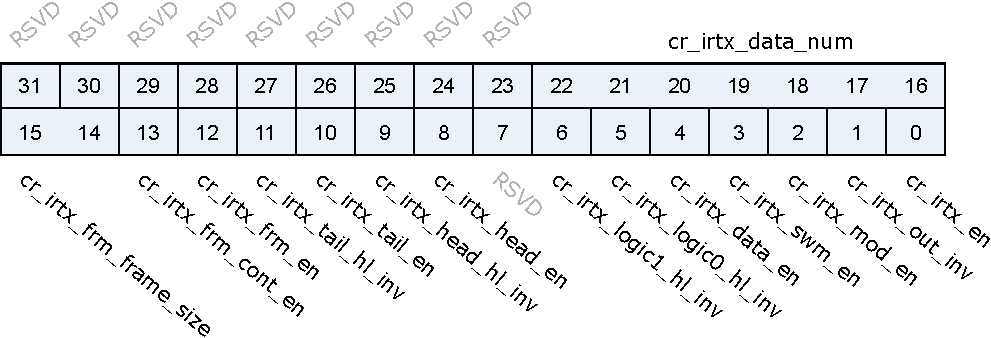
\includegraphics{ir_irtx_config.pdf}
\end{figure}

\regdes{31:18&RSVD& & & \\\hline
17:12&cr\_irtx\_data\_num&r/w&6'd31&Bit count of Data phase (unit: bit / PW for normal / SWM)\\\hline
11&cr\_irtx\_tail\_hl\_inv&r/w&1'b0&Tail pulse H/L inverse signal (Don't care if SWM is enabled) \par 0: Phase 0 is High (Active), phase 1 is Low (Idle) (H -> L) \par 1: Phase 0 is Low (Idle), phase 1 is High (Active) (L -> H)
\\\hline
10&cr\_irtx\_tail\_en&r/w&1'b1&Enable signal of tail pulse (Don't care if SWM is enabled)\\\hline
9&cr\_irtx\_head\_hl\_inv&r/w&1'b0&Tail pulse H/L inverse signal (Don't care if SWM is enabled) \par 0: Phase 0 is High (Active), phase 1 is Low (Idle) (H -> L) \par 1: Phase 0 is Low (Idle), phase 1 is High (Active) (L -> H)
\\\hline
8&cr\_irtx\_head\_en&r/w&1'b1&Enable signal of head pulse (Don't care if SWM is enabled)\\\hline
7&RSVD& & & \\\hline
6&cr\_irtx\_logic1\_hl\_inv&r/w&1'b0&Logic 1 H/L inverse signal (Don't care if SWM is enabled) \par 0: Phase 0 is High (Active), phase 1 is Low (Idle) (H -> L) \par 1: Phase 0 is Low (Idle), phase 1 is High (Active) (L -> H)
\\\hline
5&cr\_irtx\_logic0\_hl\_inv&r/w&1'b0&Logic 0 H/L inverse signal (Don't care if SWM is enabled) \par 0: Phase 0 is High (Active), phase 1 is Low (Idle) (H -> L) \par 1: Phase 0 is Low (Idle), phase 1 is High (Active) (L -> H)
\\\hline
4&cr\_irtx\_data\_en&r/w&1'b1&Enable signal of data phase (Don't care if SWM is enabled)\\\hline
3&cr\_irtx\_swm\_en&r/w&1'b0&Enable signal of IRTX Software Mode (SWM)\\\hline
2&cr\_irtx\_mod\_en&r/w&1'b0&Enable signal of output modulation\\\hline
1&cr\_irtx\_out\_inv&r/w&1'b0&Output inverse signal \par 1'b0: Output stays at Low during idle state \par 1'b1: Output stays at High during idle state
\\\hline
0&cr\_irtx\_en&r/w&1'b0&Enable signal of IRTX function \par Asserting this bit will trigger the transaction, and should be de-asserted after finish
\\\hline

}
\subsection{irtx\_int\_sts}
\label{ir-irtx-int-sts}
Address:0x4000a604
 \begin{figure}[H]
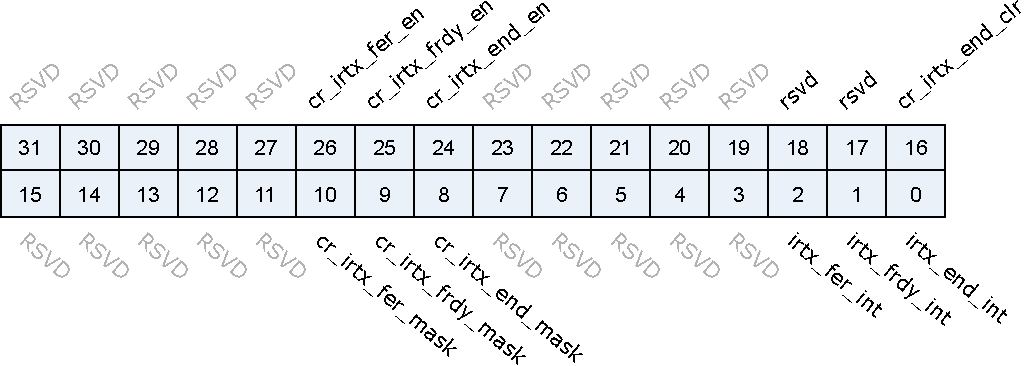
\includegraphics{ir_irtx_int_sts.pdf}
\end{figure}

\regdes{31:25&RSVD& & & \\\hline
24&cr\_irtx\_end\_en&r/w&1'b1&Interrupt enable of irtx\_end\_int\\\hline
23:17&RSVD& & & \\\hline
16&cr\_irtx\_end\_clr&w1c&1'b0&Interrupt clear of irtx\_end\_int\\\hline
15:9&RSVD& & & \\\hline
8&cr\_irtx\_end\_mask&r/w&1'b1&Interrupt mask of irtx\_end\_int\\\hline
7:1&RSVD& & & \\\hline
0&irtx\_end\_int&r&1'b0&IRTX transfer end interrupt\\\hline

}
\subsection{irtx\_data\_word0}
\label{ir-irtx-data-word0}
Address:0x4000a608
 \begin{figure}[H]
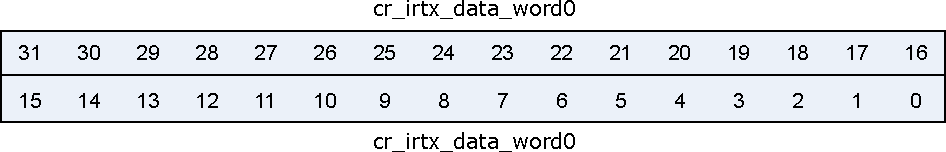
\includegraphics{ir_irtx_data_word0.pdf}
\end{figure}

\regdes{31:0&cr\_irtx\_data\_word0&r/w&32'h0&TX data word 0 (Don't care if SWM is enabled)\\\hline

}
\subsection{irtx\_data\_word1}
\label{ir-irtx-data-word1}
Address:0x4000a60c
 \begin{figure}[H]
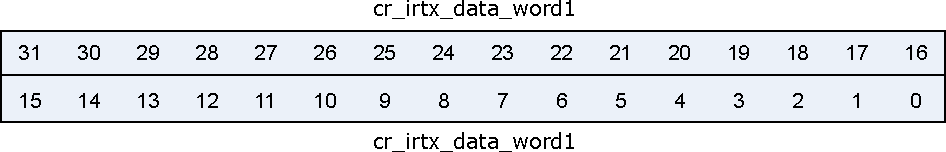
\includegraphics{ir_irtx_data_word1.pdf}
\end{figure}

\regdes{31:0&cr\_irtx\_data\_word1&r/w&32'h0&TX data word 1 (Don't care if SWM is enabled)\\\hline

}
\subsection{irtx\_pulse\_width}
\label{ir-irtx-pulse-width}
Address:0x4000a610
 \begin{figure}[H]
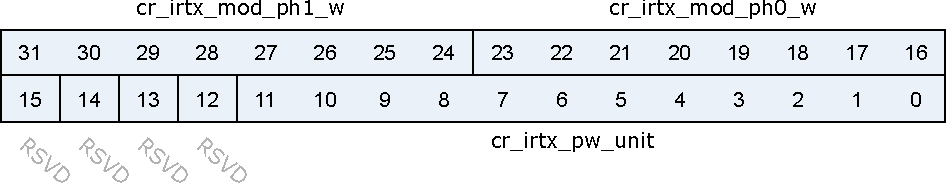
\includegraphics{ir_irtx_pulse_width.pdf}
\end{figure}

\regdes{31:24&cr\_irtx\_mod\_ph1\_w&r/w&8'd34&Modulation phase 1 width\\\hline
23:16&cr\_irtx\_mod\_ph0\_w&r/w&8'd17&Modulation phase 0 width\\\hline
15:12&RSVD& & & \\\hline
11:0&cr\_irtx\_pw\_unit&r/w&12'd1124&Pulse width unit\\\hline

}
\subsection{irtx\_pw}
\label{ir-irtx-pw}
Address:0x4000a614
 \begin{figure}[H]
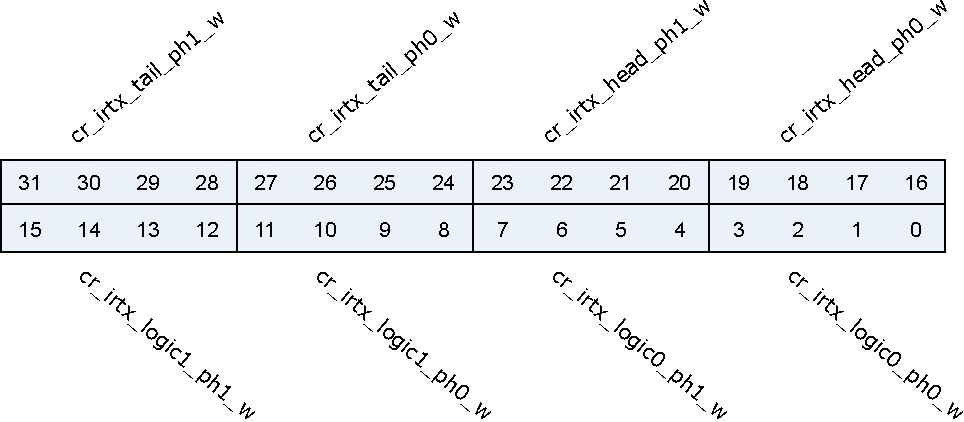
\includegraphics{ir_irtx_pw.pdf}
\end{figure}

\regdes{31:28&cr\_irtx\_tail\_ph1\_w&r/w&4'd0&Pulse width of tail pulse phase 1 (Don't care if SWM is enabled)\\\hline
27:24&cr\_irtx\_tail\_ph0\_w&r/w&4'd0&Pulse width of tail pulse phase 0 (Don't care if SWM is enabled)\\\hline
23:20&cr\_irtx\_head\_ph1\_w&r/w&4'd7&Pulse width of head pulse phase 1 (Don't care if SWM is enabled)\\\hline
19:16&cr\_irtx\_head\_ph0\_w&r/w&4'd15&Pulse width of head pulse phase 0 (Don't care if SWM is enabled)\\\hline
15:12&cr\_irtx\_logic1\_ph1\_w&r/w&4'd2&Pulse width of logic1 phase 1 (Don't care if SWM is enabled)\\\hline
11:8&cr\_irtx\_logic1\_ph0\_w&r/w&4'd0&Pulse width of logic1 phase 0 (Don't care if SWM is enabled)\\\hline
7:4&cr\_irtx\_logic0\_ph1\_w&r/w&4'd0&Pulse width of logic0 phase 1 (Don't care if SWM is enabled)\\\hline
3:0&cr\_irtx\_logic0\_ph0\_w&r/w&4'd0&Pulse width of logic0 phase 0 (Don't care if SWM is enabled)\\\hline

}
\subsection{irtx\_swm\_pw\_0}
\label{ir-irtx-swm-pw-0}
Address:0x4000a640
 \begin{figure}[H]
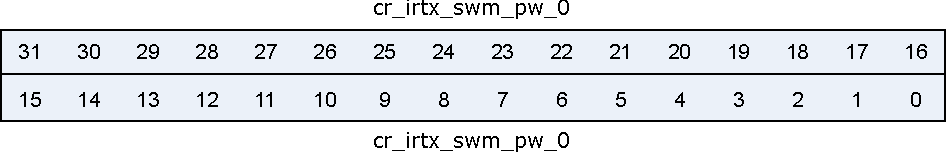
\includegraphics{ir_irtx_swm_pw_0.pdf}
\end{figure}

\regdes{31:0&cr\_irtx\_swm\_pw\_0&r/w&32'h0&IRTX Software Mode pulse width data \#0~\#7, each pulse is represented by 4-bit \par ([3:0] is the 1st pulse, [7:4] is the 2nd pulse, [11:8] is the 3rd pulse, etc)
\\\hline

}
\subsection{irtx\_swm\_pw\_1}
\label{ir-irtx-swm-pw-1}
Address:0x4000a644
 \begin{figure}[H]
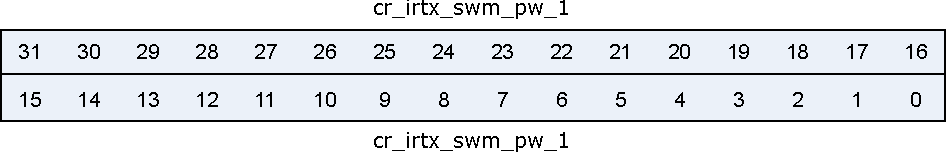
\includegraphics{ir_irtx_swm_pw_1.pdf}
\end{figure}

\regdes{31:0&cr\_irtx\_swm\_pw\_1&r/w&32'h0&IRTX Software Mode pulse width data \#8~\#15, each pulse is represented by 4-bit \par ([3:0] is the 1st pulse, [7:4] is the 2nd pulse, [11:8] is the 3rd pulse, etc)
\\\hline

}
\subsection{irtx\_swm\_pw\_2}
\label{ir-irtx-swm-pw-2}
Address:0x4000a648
 \begin{figure}[H]
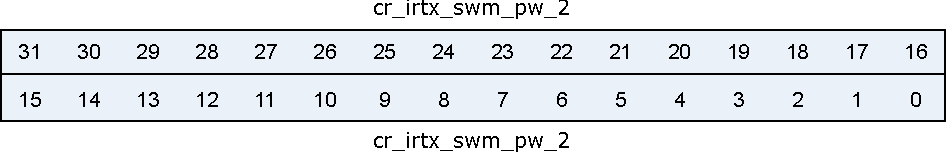
\includegraphics{ir_irtx_swm_pw_2.pdf}
\end{figure}

\regdes{31:0&cr\_irtx\_swm\_pw\_2&r/w&32'h0&IRTX Software Mode pulse width data \#16~\#23, each pulse is represented by 4-bit \par ([3:0] is the 1st pulse, [7:4] is the 2nd pulse, [11:8] is the 3rd pulse, etc)
\\\hline

}
\subsection{irtx\_swm\_pw\_3}
\label{ir-irtx-swm-pw-3}
Address:0x4000a64c
 \begin{figure}[H]
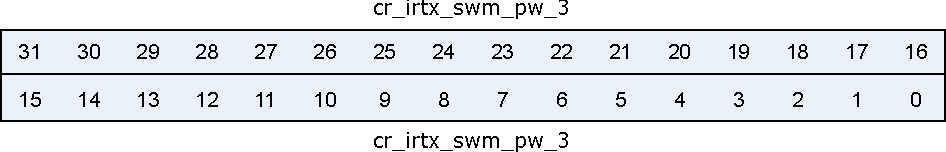
\includegraphics{ir_irtx_swm_pw_3.pdf}
\end{figure}

\regdes{31:0&cr\_irtx\_swm\_pw\_3&r/w&32'h0&IRTX Software Mode pulse width data \#24~\#31, each pulse is represented by 4-bit \par ([3:0] is the 1st pulse, [7:4] is the 2nd pulse, [11:8] is the 3rd pulse, etc)
\\\hline

}
\subsection{irtx\_swm\_pw\_4}
\label{ir-irtx-swm-pw-4}
Address:0x4000a650
 \begin{figure}[H]
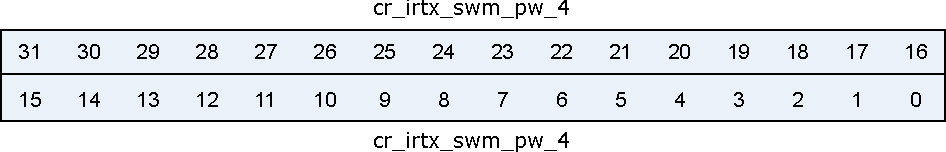
\includegraphics{ir_irtx_swm_pw_4.pdf}
\end{figure}

\regdes{31:0&cr\_irtx\_swm\_pw\_4&r/w&32'h0&IRTX Software Mode pulse width data \#32~\#39, each pulse is represented by 4-bit \par ([3:0] is the 1st pulse, [7:4] is the 2nd pulse, [11:8] is the 3rd pulse, etc)
\\\hline

}
\subsection{irtx\_swm\_pw\_5}
\label{ir-irtx-swm-pw-5}
Address:0x4000a654
 \begin{figure}[H]
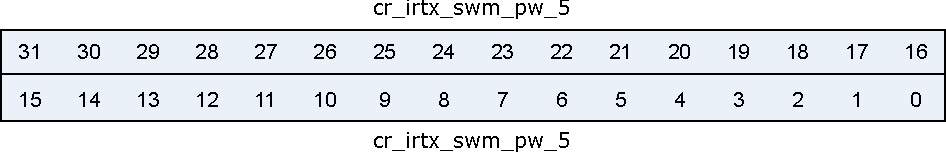
\includegraphics{ir_irtx_swm_pw_5.pdf}
\end{figure}

\regdes{31:0&cr\_irtx\_swm\_pw\_5&r/w&32'h0&IRTX Software Mode pulse width data \#40~\#47, each pulse is represented by 4-bit \par ([3:0] is the 1st pulse, [7:4] is the 2nd pulse, [11:8] is the 3rd pulse, etc)
\\\hline

}
\subsection{irtx\_swm\_pw\_6}
\label{ir-irtx-swm-pw-6}
Address:0x4000a658
 \begin{figure}[H]
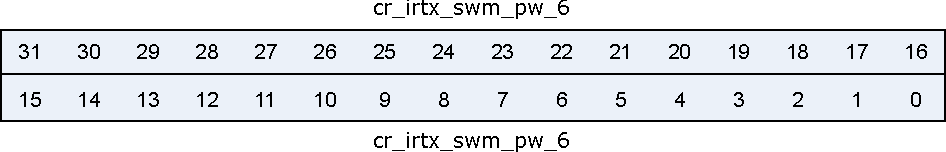
\includegraphics{ir_irtx_swm_pw_6.pdf}
\end{figure}

\regdes{31:0&cr\_irtx\_swm\_pw\_6&r/w&32'h0&IRTX Software Mode pulse width data \#48~\#55, each pulse is represented by 4-bit \par ([3:0] is the 1st pulse, [7:4] is the 2nd pulse, [11:8] is the 3rd pulse, etc)
\\\hline

}
\subsection{irtx\_swm\_pw\_7}
\label{ir-irtx-swm-pw-7}
Address:0x4000a65c
 \begin{figure}[H]
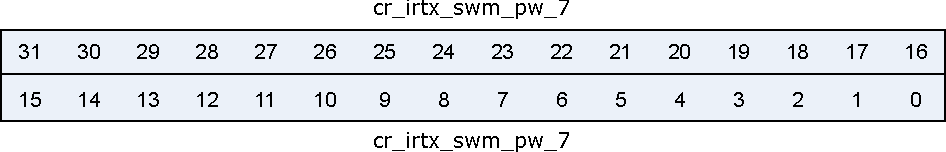
\includegraphics{ir_irtx_swm_pw_7.pdf}
\end{figure}

\regdes{31:0&cr\_irtx\_swm\_pw\_7&r/w&32'h0&IRTX Software Mode pulse width data \#56~\#63, each pulse is represented by 4-bit \par ([3:0] is the 1st pulse, [7:4] is the 2nd pulse, [11:8] is the 3rd pulse, etc)
\\\hline

}
\subsection{irrx\_config}
\label{ir-irrx-config}
Address:0x4000a680
 \begin{figure}[H]
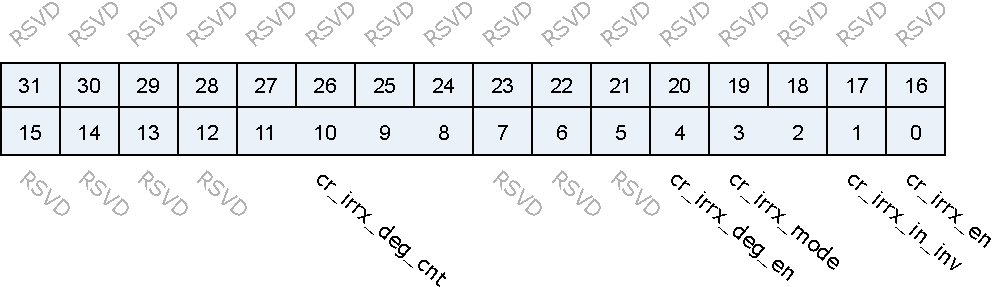
\includegraphics{ir_irrx_config.pdf}
\end{figure}

\regdes{31:12&RSVD& & & \\\hline
11:8&cr\_irrx\_deg\_cnt&r/w&4'd0&De-glitch function cycle count\\\hline
7:5&RSVD& & & \\\hline
4&cr\_irrx\_deg\_en&r/w&1'b0&Enable signal of IRRX input de-glitch function\\\hline
3:2&cr\_irrx\_mode&r/w&2'd0&IRRX mode \par 0: NEC \par 1: RC5 \par 2: SW pulse-width detection mode (SWM) \par 3: Reserved
\\\hline
1&cr\_irrx\_in\_inv&r/w&1'b1&Input inverse signal\\\hline
0&cr\_irrx\_en&r/w&1'b0&Enable signal of IRRX function \par Asserting this bit will trigger the transaction, and should be de-asserted after finish
\\\hline

}
\subsection{irrx\_int\_sts}
\label{ir-irrx-int-sts}
Address:0x4000a684
 \begin{figure}[H]
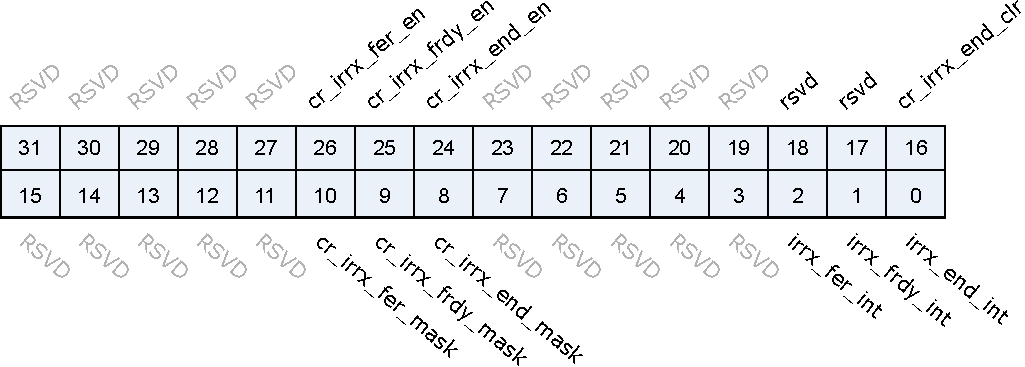
\includegraphics{ir_irrx_int_sts.pdf}
\end{figure}

\regdes{31:25&RSVD& & & \\\hline
24&cr\_irrx\_end\_en&r/w&1'b1&Interrupt enable of irrx\_end\_int\\\hline
23:17&RSVD& & & \\\hline
16&cr\_irrx\_end\_clr&w1c&1'b0&Interrupt clear of irrx\_end\_int\\\hline
15:9&RSVD& & & \\\hline
8&cr\_irrx\_end\_mask&r/w&1'b1&Interrupt mask of irrx\_end\_int\\\hline
7:1&RSVD& & & \\\hline
0&irrx\_end\_int&r&1'b0&IRRX transfer end interrupt\\\hline

}
\subsection{irrx\_pw\_config}
\label{ir-irrx-pw-config}
Address:0x4000a688
 \begin{figure}[H]
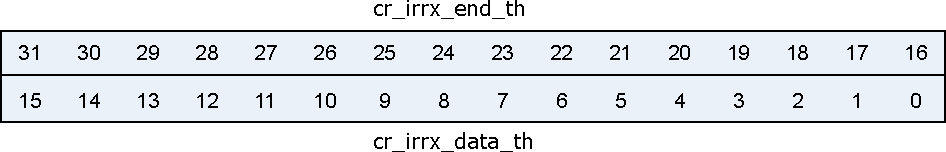
\includegraphics{ir_irrx_pw_config.pdf}
\end{figure}

\regdes{31:16&cr\_irrx\_end\_th&r/w&16'd8999&Pulse width threshold to trigger END condition\\\hline
15:0&cr\_irrx\_data\_th&r/w&16'd3399&Pulse width threshold for Logic0/1 detection (Don't care if SWM is enabled)\\\hline

}
\subsection{irrx\_data\_count}
\label{ir-irrx-data-count}
Address:0x4000a690
 \begin{figure}[H]
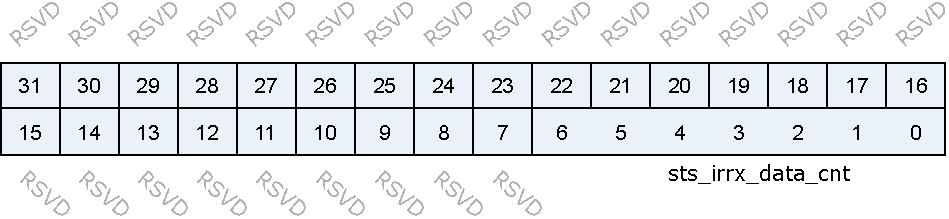
\includegraphics{ir_irrx_data_count.pdf}
\end{figure}

\regdes{31:7&RSVD& & & \\\hline
6:0&sts\_irrx\_data\_cnt&r&7'd0&RX data bit count (pulse-width count for SWM)\\\hline

}
\subsection{irrx\_data\_word0}
\label{ir-irrx-data-word0}
Address:0x4000a694
 \begin{figure}[H]
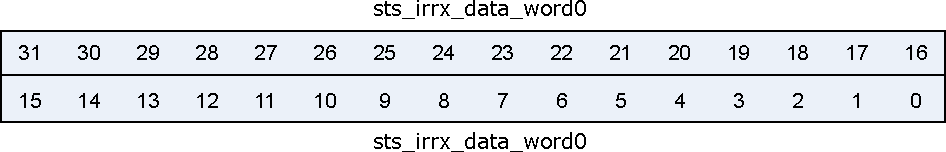
\includegraphics{ir_irrx_data_word0.pdf}
\end{figure}

\regdes{31:0&sts\_irrx\_data\_word0&r&32'h0&RX data word 0\\\hline

}
\subsection{irrx\_data\_word1}
\label{ir-irrx-data-word1}
Address:0x4000a698
 \begin{figure}[H]
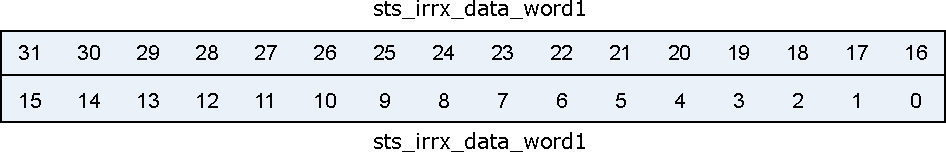
\includegraphics{ir_irrx_data_word1.pdf}
\end{figure}

\regdes{31:0&sts\_irrx\_data\_word1&r&32'h0&RX data word 1\\\hline

}
\subsection{irrx\_swm\_fifo\_config\_0}
\label{ir-irrx-swm-fifo-config-0}
Address:0x4000a6c0
 \begin{figure}[H]
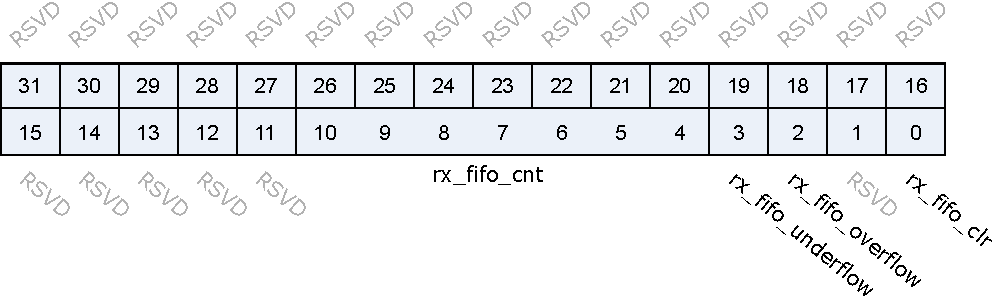
\includegraphics{ir_irrx_swm_fifo_config_0.pdf}
\end{figure}

\regdes{31:11&RSVD& & & \\\hline
10:4&rx\_fifo\_cnt&r&7'd0&RX FIFO available count\\\hline
3&rx\_fifo\_underflow&r&1'b0&Underflow flag of RX FIFO, can be cleared by rx\_fifo\_clr\\\hline
2&rx\_fifo\_overflow&r&1'b0&Overflow flag of RX FIFO, can be cleared by rx\_fifo\_clr\\\hline
1&RSVD& & & \\\hline
0&rx\_fifo\_clr&w1c&1'b0&Clear signal of RX FIFO\\\hline

}
\subsection{irrx\_swm\_fifo\_rdata}
\label{ir-irrx-swm-fifo-rdata}
Address:0x4000a6c4
 \begin{figure}[H]
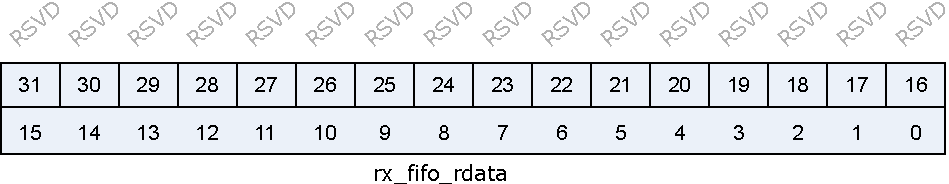
\includegraphics{ir_irrx_swm_fifo_rdata.pdf}
\end{figure}

\regdes{31:16&RSVD& & & \\\hline
15:0&rx\_fifo\_rdata&r&16'h0&IRRX Software Mode pulse width data\\\hline

}
